\documentclass[12pt]{article}
\usepackage{graphicx}
\usepackage{amsmath}
\usepackage{verbatim}
\begin{document}

\begin{titlepage}
\title{
Report on Analytic Solution for Annular Ducts}


\author{ Jeff Severino
 \\
University of Toledo \\
Toledo, OH  43606 \\
email: jseveri@rockets.utoledo.edu  }

\maketitle

\end{titlepage}

\section{Current Research Direction}
 The goal is to currently compute the coefficients $A$ and $B$, the weighting
 factors for the Bessel Functions for the first and second kind. V072
 contains FORTRAN subroutines that compute these along with the Bessel functions.
 \section{Numerical Computation of Annular Duct Modes}

  
\section{Research Performed This Week}
\subsection{Theoretical Background}

The analytic radial mode shape is of the form,

\begin{equation}
    R_m(k_{r,mn} r) =  A J_m (k_{r,mn} r) + B Y_m (k_{r,nmn} r)
\end{equation}
The key to the numerical procedure is the following ``transcendental'' equation,
\begin{equation}
    \begin{vmatrix}
        J'_m(k_{r,mn} r_H) &Y'_m(k_{r,mn} r_H) \\
        J'_m(k_{r,mn} r_T) &Y'_m(k_{r,mn} r_T) 
    \end{vmatrix}   
    = 0
\end{equation}
 The non-dimensional roots $k_{r,mn} r_T$ are found using initial guess and then incrementing from there

 \begin{equation}
     k_{r,mn} = 
    \begin{cases}
        m & \text{if } n = 1\\
        k_{r,m(n-1)} r_T + \pi,              & \text{if }  n > 1.
    \end{cases}
 \end{equation}

 The estimate is refined by incrementing the value of $k_{r,mn}$ by $\pi/10$ until
 the determinant above changes sign. The step size is then halved and also changes 
 sign. This iterative process continues until the absolute value of the determinant 
 is reduced to a preassigned value (error tolerance?). The non dimensional versions
 of these equations are used in the FORTRAN 77 Code.

 Once $k_{r,mn}$ has been computed, the weighting factors $A$ and $B$ are assigned to 
 one of the following two sets of values ( \verb|eigen.f|)


 The remainder of the procedure is being documented along with directions on 
 how to pass in the correct inputs to the F77 calls
 The estimate is refined by incrementing the value of $k_{r,mn}$ by $\pi/10$ until
 the determinant above changes sign. The step size is then halved and also changes 
 sign. This iterative process continues until the absolute value of the determinant 
 is reduced to a preassigned value (error tolerance?). The non dimensional versions
 of these equations are used in the FORTRAN 77 Code, \verb|anrt.f|, which calls 
 \verb|anfu.f|.

 Once $k_{r,mn}$ has been computed, the weighting factors $A$ and $B$ are assigned to 
 one of the following two sets of values ( \verb|eigen.f|)
 \begin{equation*}
     \begin{cases}
         A = 1 \\ 
         B = - \frac{J'_m(k_{r,mn} r_H )}{Y'_m(k_{r,mn} r_H )}
     \end{cases}
     \text{or,}
     \begin{cases}
         A =- \frac{Y'_m(k_{r,mn} r_H )}{J'_m(k_{r,mn} r_H )}  \\
         B = 1
     \end{cases}
 \end{equation*}
Of these two values, which ever has the smaller $A^2 + B^2$ is chosen.

The desired normalization,

\begin{equation}
    \int_{r_T}^{r_H} R_m^2(k_{r,mn} r) r dr = \frac{1}{2}\left( r_T^2-r_H^2 \right)
    \label{eqn:desirednormalization}
\end{equation}

is obtained by computing the value on the left-hand side of 
Equation (\ref{eqn:desirednormalization}) using the expression,

\begin{equation}
    \int_{r_H}^{r_T} R_m^2(k_{r,mn} r) r dr = 
    \frac{1}{2}\left( r^2 - \frac{m^2}{k_{r,mn}^2} \right)R_m^2 (k_{r,mn} r)\Big|_{r = r_H}^{r_T} \equiv C
\end{equation}

The constants $A$ and $B$ are divided by,

\begin{equation}
    \sqrt{\frac{2C}{\left( r_T^2 - r_H^2 \right)}}
    \label{eqn:normalizationconst}
\end{equation}
to give the normalization needed in Equation (\ref{eqn:desirednormalization}) 

The non-dimensionalization in this code uses the following,
\[ X_{mn} = k_{r,mn} r_T\]
\[ x = r/r_T\]
\[ \sigma = r_H/r_T\]

The non-dimensional equivalent expressions are 

\begin{equation}
    \int_{\sigma}^{1} R_m^2(X_{mn} x) x dr = \frac{1}{2}\left( 1 - \sigma^2 \right)
    \label{eqn:desirednormalization_nondimensional}
\end{equation}

\begin{equation}
    \int_{\sigma}^{1} R_m^2(X_{mn} x) x dr = 
    \frac{1}{2}\left( x^2 - \frac{m^2}{X_{mn}^2} \right)R_m^2 (X_{mn} x)\Big|_{x = \sigma}^{1}
\end{equation}
and the constant that A and B are divided by becomes 

\begin{equation}
    \sqrt{\frac{
\left( 1 - \frac{m^2}{X_{mn}^2} \right)R_m^2 (X_{mn} )  -
\left( \sigma^2 - \frac{m^2}{X_{mn}^2} \right)R_m^2 (X_{mn} \sigma)
}{\left( 1 - \sigma^2 \right)}}
    \label{eqn:normalizationconst_nondimension}
\end{equation}
\begin{itemize}
    \item \verb|eigen.f|, 
        \subitem Computes the weighting factors, $A$ and $B$ for the radial mode
        shpe
    \item \verb|besj.f|, 
        \subitem Computes the bessel functions of the first kind and their derivatives
        of positive or zero order, n, and zero or positive argument x 
    \item \verb|besy.f|, and 
        \subitem Computes the bessel function of the second kind and their 
        derivatives of positive or zero order, n, and zero or positive argument x 
    \item \verb|rmode.f|. 
        \subitem Calculate radial mode shape psi for the (m,n) radial mode of an annular duct 
\end{itemize}


\section{Issues and Concerns}
The mode shapes produced do not have zero slope at the boundaries.

Currently a subdirectory within the \verb|v070_nasalib| directory has a testing 
code to obtain the annular duct modes. 

The current code is, 
\begin{verbatim}

! Notes:
! Pros of f90 for V072:
!   better management of inputs and outputs
!       - explicit interfaces
PROGRAM BesselFunctionCode
      USE, INTRINSIC :: ISO_FORTRAN_ENV  
      IMPLICIT NONE
      INTEGER, PARAMETER :: &
          rDef = REAL64, &
          numberOfGridPoints = 1000

      INTEGER :: &
          UNIT                  ,&
          azimuthal_mode_number ,&
          radial_mode_number    ,&
          i
      
      
      REAL(KIND=rDef) :: & 
          r_min, &
          r_max, &
          dr,  &
          AMN, &
          BMN, &
          hubTipRatio,&
          convergence_criteria ,& 
          PSI

      REAL(KIND=rDef), DIMENSION(:), ALLOCATABLE :: X

      REAL(KIND=rDef),DIMENSION(2) :: IERROR1, IERROR2
      REAL(KIND=rDef),DIMENSION(4) :: anfu_bessel_function_error 

      REAL(KIND=rDef) ::  anrt_convergence_flag 
      
      REAL(KIND=rDef) :: non_dimensional_roots


      ALLOCATE(X(numberOfGridPoints))

      ! Notes:
      ! r_min cant be zero 

      r_min = 0.20_rDef 
      r_max = 3.0_rDef      

      hubTipRatio = r_min/r_max 

      dr    = (r_max-r_min)/REAL(numberOfGridPoints-1, rDef)

      DO i =1,numberOfGridPoints

      X(i)  = (r_min+REAL(i-1, rDef)*dr)/r_max !radial grid
      
      
      ENDDO


      azimuthal_mode_number = 2 
      radial_mode_number = 1
      convergence_criteria = 1.0E-5_rDef
      
      
      CALL ANRT(&
          azimuthal_mode_number,&
          radial_mode_number,&
          hubTipRatio,&
          convergence_criteria,&
          non_dimensional_roots,&
          anfu_bessel_function_error,&
          anrt_convergence_flag)

      WRITE(0,*) 'k_mn=' ,non_dimensional_roots

      IF (anrt_convergence_flag .gt. 0.0_rDef) THEN
          WRITE(0,*) 'ERROR: ANRT DID NOT CONVERGE ',anrt_convergence_flag
      ELSE
      ENDIF

      ! STOP
      ! Obtaining A and B coefficients for radial mode shape
      CALL EIGEN(&
          azimuthal_mode_number, &
          hubTipRatio               , &
          non_dimensional_roots                  , &
          AMN                  , &
          BMN                  , &
          IERROR1)

      ! in the case of cylindrical ducts...
      ! AMN = 1.0_rDef
      ! BMN = 0.0_rDef
      WRITE(0,*) 'A =' , AMN
      WRITE(0,*) 'B =' , BMN
      WRITE(0,*) 'non_dimensional_roots =' , non_dimensional_roots
      OPEN(NEWUNIT=UNIT,FILE='radial_mode_data.dat') 
      WRITE(UNIT,*) 'radius ', 'pressure '
       
      DO i = 1,numberOfGridPoints

      CALL RMODE(&
      azimuthal_mode_number,&
      X(i),&
      AMN,&
      BMN,&
      PSI,&
      IERROR2)
  
      WRITE(UNIT,*) X(i), PSI

      ENDDO
      CLOSE(UNIT)

END PROGRAM
\end{verbatim}
This produces the following:

\begin{figure}
    \centering
    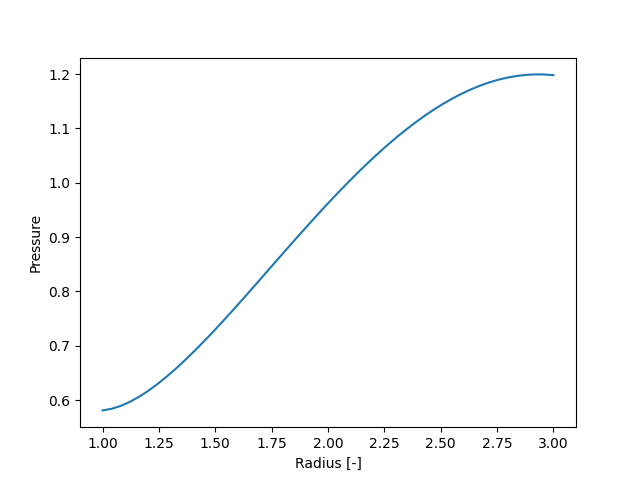
\includegraphics{figures/Figure_1_1.png}
    \caption{initial result}
    \label{fig:dd}
\end{figure}



Figure \ref{fig:dd} does not have zero slope boundaries as expected for a hard 
wall.

\section{Planned Research} 
Come up with sanity checks to test the functionality of this testing code.

I can compare bessel function plots in python to the output in F77 to see if they are identical\dots.
 \end{document}
